\onehalfspacing
\section{Đề số 16}
\graphicspath{{./img/}}
\begin{bt} 
    \hfill
	\begin{enumerate}[a.]
		\item Tính: $A=1 \frac{13}{15} \cdot(0,5)^2 \cdot 3+\left(\frac{8}{15}-1 \frac{19}{60}\right): 1 \frac{23}{24}$
        \item So sánh: $16^{20}$ và $2^{100}$
	\end{enumerate}
	\loigiai{
        \begin{enumerate}
            \item Biến đổi:\\[5pt]
            $A =\frac{7}{5}-\frac{47}{60}: \frac{47}{24} 
              = \frac{7}{5}-\frac{2}{5} 
              = 1$
            \item + Biến đổi: $16^{20}=2^{4.20}=2^{80}$\\[5pt]
            + Có $2^{80}<2^{100}$ vì $(1<2 ; 80<100)$\\[5pt]
            Vậy $16^{20}<2^{100}$
        \end{enumerate}
    } 
\end{bt}

\begin{bt}
	\hfill
	\begin{enumerate}[a.]
		\item Tìm $x$ biết: $|2 x-7|+\frac{1}{2}=1 \frac{1}{2}$
        \item Tìm số tự nhiên $\mathrm{n}$ biết: $3^{-1} \cdot 3^n+4 \cdot 3^n=13.3^5$
	\end{enumerate}
	\loigiai{
        \begin{enumerate}
            \item Ta có $|2 x-7|+\frac{1}{2}=1 \frac{1}{2}=|2 x-7|=1 \\[5pt]
            \Rightarrow 2 x-7=1 \text { hoặc } 2 x-7=-1 \\[5pt]
            \Rightarrow x=4 \text { hoặc } x=3 \\[5pt]
            \text { Vậy } x=4 \text { hoặc } x=3 \text {. }$
            \item Biến đổi được $3^n \cdot\left(3^{-1}+4\right)=13.3^5 \\[5pt]
            \Rightarrow 3^n=3^6 \\[5pt]
            \Rightarrow \mathrm{n}=6 \\[5pt]
            \text { KL: Vậy } \mathrm{n}=6$
        \end{enumerate}
    } 
\end{bt}

\begin{bt}
	\hfill
	\begin{enumerate}[a.]
		\item Cho dãy tỉ số bằng nhau: $\frac{2 a+b+c+d}{a}=\frac{a+2 b+c+d}{b}=\frac{a+b+2 c+d}{c}=\frac{a+b+c+2 d}{d}$ Tính giá trị biểu thức $\mathrm{Q}$, biết $\mathrm{Q}=\frac{a+b}{c+d}+\frac{b+c}{d+a}+\frac{c+d}{a+b}+\frac{d+a}{b+c}$
        \item Cho biểu thức $M=\frac{x}{x+y+z}+\frac{y}{x+y+t}+\frac{z}{y+z+t}+\frac{t}{x+z+t}$ với $x, y, z, t$ là các số tự nhiên khác 0 . Chứng minh $M^{10}<1025$.
    \end{enumerate}
	\loigiai{
        \begin{enumerate}
            \item + Biến đổi: $\frac{2 a+b+c+d}{a}=\frac{a+2 b+c+d}{b}=\frac{a+b+2 c+d}{c}=\frac{a+b+c+2 d}{d} \\[5pt]
            \frac{2 a+b+c+d}{a}-1=\frac{a+2 b+c+d}{b}-1=\frac{a+b+2 c+d}{c}-1=\frac{a+b+c+2 d}{d}-1 \\[5pt]
            \frac{a+b+c+d}{a}=\frac{a+b+c+d}{b}=\frac{a+b+c+d}{c}=\frac{a+b+c+d}{d}$\\ [5pt]
            + Nếu $a+b+c+d \neq 0$ thì $a=b=c=d \Rightarrow Q=1+1+1+1=4$ \\[5pt]
            + Nếu $a+b+c+d=0$ \\[5pt]
            thì $a+b=-(c+d) ; b+c=-(d+a) ; c+d=-(a+b) ; d+a=-(b+c)$ \\[5pt]
            $\Rightarrow Q=(-1)+(-1)+(-1)+(-1)=-4$ \\[5pt]
            + KL :\\[5pt]
            $Q=4$ khi $a+b+c+d \neq 0$ \\[5pt]
            $Q=-4$ khi $a+b+c+d=0$
            \item
            + Ta có: $\frac{x}{x+y+z}<\frac{x}{x+y} \\[5pt]
            \frac{y}{x+y+t}<\frac{y}{x+y} \\[5pt]
            \frac{z}{y+z+t}<\frac{z}{z+t} \\[5pt]
            \frac{t}{x+z+t}<\frac{t}{z+t} \\[5pt]
            \Rightarrow \mathrm{M}<\left(\frac{\mathrm{x}}{\mathrm{x}+\mathrm{y}}+\frac{\mathrm{y}}{\mathrm{x}+\mathrm{y}}\right)+\left(\frac{\mathrm{z}}{\mathrm{z}+\mathrm{t}}+\frac{\mathrm{t}}{\mathrm{z}+\mathrm{t}}\right) \Rightarrow \mathrm{M}<2 \\[5pt]
            + \text {Có } \mathrm{M}^{10}<2^{10} (\text{ Vì M}>0) \text { mà } 2^{10}=1024<1025 \\[5pt]
            \text {Vậy } \mathrm{M}^{10}<1025$
        \end{enumerate}
    }
\end{bt}

\begin{bt}
    \hfil
    \begin{enumerate}[1.]
        \item Cho tam giác $A B C$ vuông cân tại $A$. Gọi $M$ là trung điểm $B C, D$ là điểm thuộc đoạn $\mathrm{BM}$ ( $\mathrm{D}$ khác $\mathrm{B}$ và $\mathrm{M})$. Kẻ các đường thẳng $\mathrm{BH}, \mathrm{CI}$ lần lượt vuông góc với đường thẳng $\mathrm{AD}$ tại $\mathrm{H}$ và $\mathrm{I}$. Chứng minh rằng:
        \begin{enumerate}
            \item $\mathrm{BAM}=\mathrm{ACM}$ và $\mathrm{BH}=\mathrm{AI}$.
            \item Tam giác MHI vuông cân.
        \end{enumerate}   
        \item Cho tam giác $\mathrm{ABC}$ có góc $\hat{\mathrm{A}}=90^{\circ}$. Kẻ $\mathrm{AH}$ vuông góc với $\mathrm{BC}$ (H thuộc $\mathrm{BC}$ ). Tia phân giác của góc $\mathrm{HAC}$ cắt cạnh $\mathrm{BC}$ ở điểm $\mathrm{D}$ và tia phân giác của góc $\mathrm{HAB}$ cắt cạnh $\mathrm{BC}$ ở $\mathrm{E}$. Chứng minh rằng $\mathrm{AB}+\mathrm{AC}=\mathrm{BC}+\mathrm{DE}$.
    \end{enumerate}
\loigiai{
    \begin{enumerate}[1.]
        \item 
        $$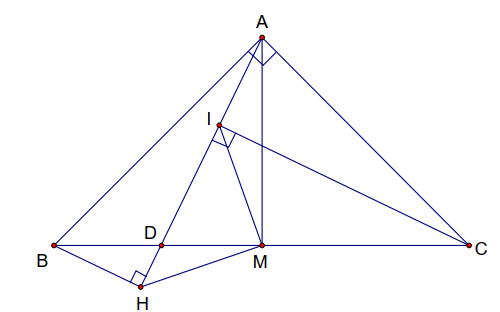
\includegraphics[width=0.57\textwidth]{16-4-lg.png}$$
        \begin{enumerate}
            \item 
            * Chứng minh: $B A M=A C M$\\[5pt]
            + Chứng minh được: $\triangle \mathrm{ABM}=\Delta \mathrm{ACM}(\mathrm{c}-\mathrm{c}-\mathrm{c})$ \\[5pt]
            + Lập luận được:$ B A M=C A M=45^{\circ}$ \\[5pt]
            +Tính ra được $A C M=45^{\circ}$ \\[5pt]
            $\Rightarrow BAM=ACM$ \\[5pt]
            * Chứng minh: $\mathrm{BH}=\mathrm{AI}$. \\[5pt]
            + Chỉ ra: $B A H=A C I$(cùng phụ $D A C$) \\[5pt]
            +Chứng minh được $\triangle \mathrm{AIC}=\Delta \mathrm{BHA}(\text { Cạnh huyền - góc nhọn) }$ \\[5pt]
            $\Rightarrow BH = AI$ (2 cạnh tương ứng) 
            \item Tam giác MHI vuông cân.\\[5pt]
            + Chứng minh được $A M \perp B C$\\[5pt]
            + Chứng minh được $\mathrm{AM}=\mathrm{MC}$\\[5pt]
            + Chứng minh được $H A M=I C M$\\[5pt]
            + Chứng minh được $\triangle \mathrm{HAM}=\Delta \mathrm{ICM}$ (c-g-c)\\[5pt]
            $\Rightarrow \mathrm{HM}=\mathrm{MI}$ (*)\\[5pt]
            + Do $\triangle \mathrm{HAM}=\triangle \mathrm{ICM} \Rightarrow H M A=I M C \Rightarrow H M B=I M A$ (do $A M B=A M C=90^{\circ}$\\[5pt]
            + Lập luận được: $H M I=90^{\circ}$
            $(* *)$\\[5pt]
            Từ $\left({ }^*\right)$ và $\left({ }^{* *}\right)=>\Delta \mathrm{MHI}$ vuông cân\\[5pt]
         \end{enumerate}
        \item 
         $$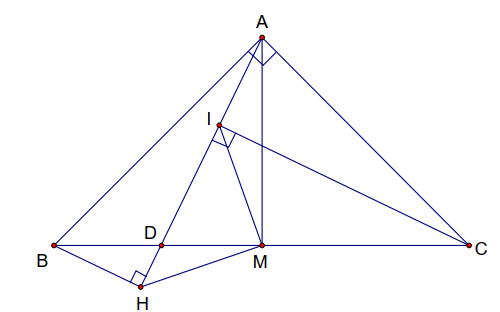
\includegraphics[width=0.57\textwidth]{16-4-lg.png}$$
         + Chứng minh được :
$$
A E \mathrm{C}=A B C+B A E=H A D+D A C+B A E=E A H+H A D+D A C=E A C
$$
(Vì $B$ và $H A C$ cùng phụ với $B A H$ )\\
Suy ra tam giác $\mathrm{AEC}$ cân tại $\mathrm{C} \Rightarrow \mathrm{AC}=\mathrm{CE}$ $\left({ }^{*}\right)$\\
+ Tương tự chứng minh được $\mathrm{AB}=\mathrm{BD}$
$\left({ }^{* *}\right)$\\
+ Từ $\left({ }^{*}\right)$ và $\left({ }^{* *}\right)$ $\Rightarrow \mathrm{AB}+\mathrm{AC}=\mathrm{BD}+\mathrm{EC}=\mathrm{ED}+\mathrm{BC}$
    \end{enumerate}
}
\end{bt}

\begin{bt}
    Cho $\mathrm{x}, \mathrm{y}, \mathrm{z}$ là 3 số thực tùy ý thỏa mãn $\mathrm{x}+\mathrm{y}+\mathrm{z}=0$ và $-1 \leq x \leq 1,-1 \leq y \leq 1$, $-1 \leq z \leq 1$. Chứng minh rằng đa thức $x^2+y^4+z^6$ có giá trị không lớn hơn 2 .
\loigiai{
     $\text { +) Trong ba số } \mathrm{x}, \mathrm{y}, \mathrm{z} \text { có ít nhất hai số cùng dấu. Giả sử } \mathrm{x} ; \mathrm{y} \geq 0 \\
     \Rightarrow \mathrm{z}=-\mathrm{x}-\mathrm{y} \leq 0 \\
     +)\mathrm{Vì } -1 \leq x \leq 1,-1 \leq y \leq 1,-1 \leq z \leq 1=>x^2+y^4+z^6 \leq|x|+|y|+|z| \\
     \Rightarrow x^2+y^4+z^6 \leq x+y-z \\
     \Rightarrow x^2+y^4+z^6 \leq-2 z \\
     +)-1 \leq z \leq 1 \text { và } \mathrm{z} \leq 0=>x^2+y^4+z^6 \leq 2 \\
     \text { KL: Vậy } x^2+y^4+z^6 \leq 2$
        
}
\end{bt}

